%
%
%

\chapter{Introduction, Review}

%%%%** Section 1
\section{Problem Statement and Learning Objectives}

Be able to
\begin{itemize}
    \item Know pre-requisite mathematical concepts for the course including
    \begin{itemize}
        \item Linear Ordinary Differential Equations
        \item Laplace Transform
        \item Partial Fraction Expansion
        \item Linearization
    \end{itemize}
    \item Compute forward and inverse Laplace Transform of several basic time functions into the $s=\sigma+j\omega$ domain.
    \item Convert a rational polynomial in $s$ to the partial fraction expansion (for simple cases).
    \item Explain the envelope and sinusoidal components of the time response of a system with complex poles.
    \item Compute a linearized version of a non-linear function about a specified point where it is smooth and differentiable.
    \item compute a LODE by linearizing a non-linear differential equation about a specified point where it is smooth and differentiable.
\end{itemize}


\subsection{Overview of Control System Engineering}


In this course we will learn how to design control systems using basic, but still widely used techniques.
Control systems are necessary because systems such as transportation vehicles, heating and air conditioning systems,
heart-lung machines, and many other examples, do not always give the same output for a given input.  For example,
if you push the accelerator of a car to a specific angle from the floor boards, the car could go at a variety of speeds
depending on external factors such as load, wind, or whether you are driving up a mountain.   Temperature control of a room
might depend on the outside temperature, sunshine, etc.   The most widely used approach to these problems is to
return a measurement of the {\it actual } quantity (speed, temperature, etc.) back to the controller and change the
commanded input based on the {\it error} between desired and actual quantities.    This is termed ``negative feedback"
because of the subtraction inherent in computing the error.

Design of a control system is a multi-stepped process which first requires a detailed analysis of the dynamics of
the system being controlled (Figure \ref{fig_control_design_flow}).  The process starts with identification of parts belonging
to the physical system (which we will later call the ``plant"), and proceeds to making a schematic model of
how the parts are interconnected.   The parameters of this model (called ``lumped" parameters because each element
occupies a point in space like a point-mass), are quantities like mass, resistance, spring constant, capacitance, etc.
From the lumped physical model, we derive differential equations using laws such as Kirchoff's laws or Newton's laws.
In many real-world systems, the differential equations are non-linear, but many more mathematical techniques are available
for systems of linear ordinary differential equations (LODEs).  We can use the process of {\it linearization} to generate  LODEs
that {\it approximate} the non-linear equations.    Finally, we create a mathematical model suited to control system design.
There are two main mathematical formulations of such models, Classical/Laplace transfer functions, and State Space models.

Classical models are transfer functions based on use of the Laplace transform to convert LODEs into polynomials or ratios
of polynomials.   State Space models stay in the time domain and map a system of LODEs into a matrix version of a first-order
LODE.

The rest of this book will cover this process for the first 4 Chapters.  Then we will start designing controllers themselves
in Chapters 5-11.

\begin{figure}\centering
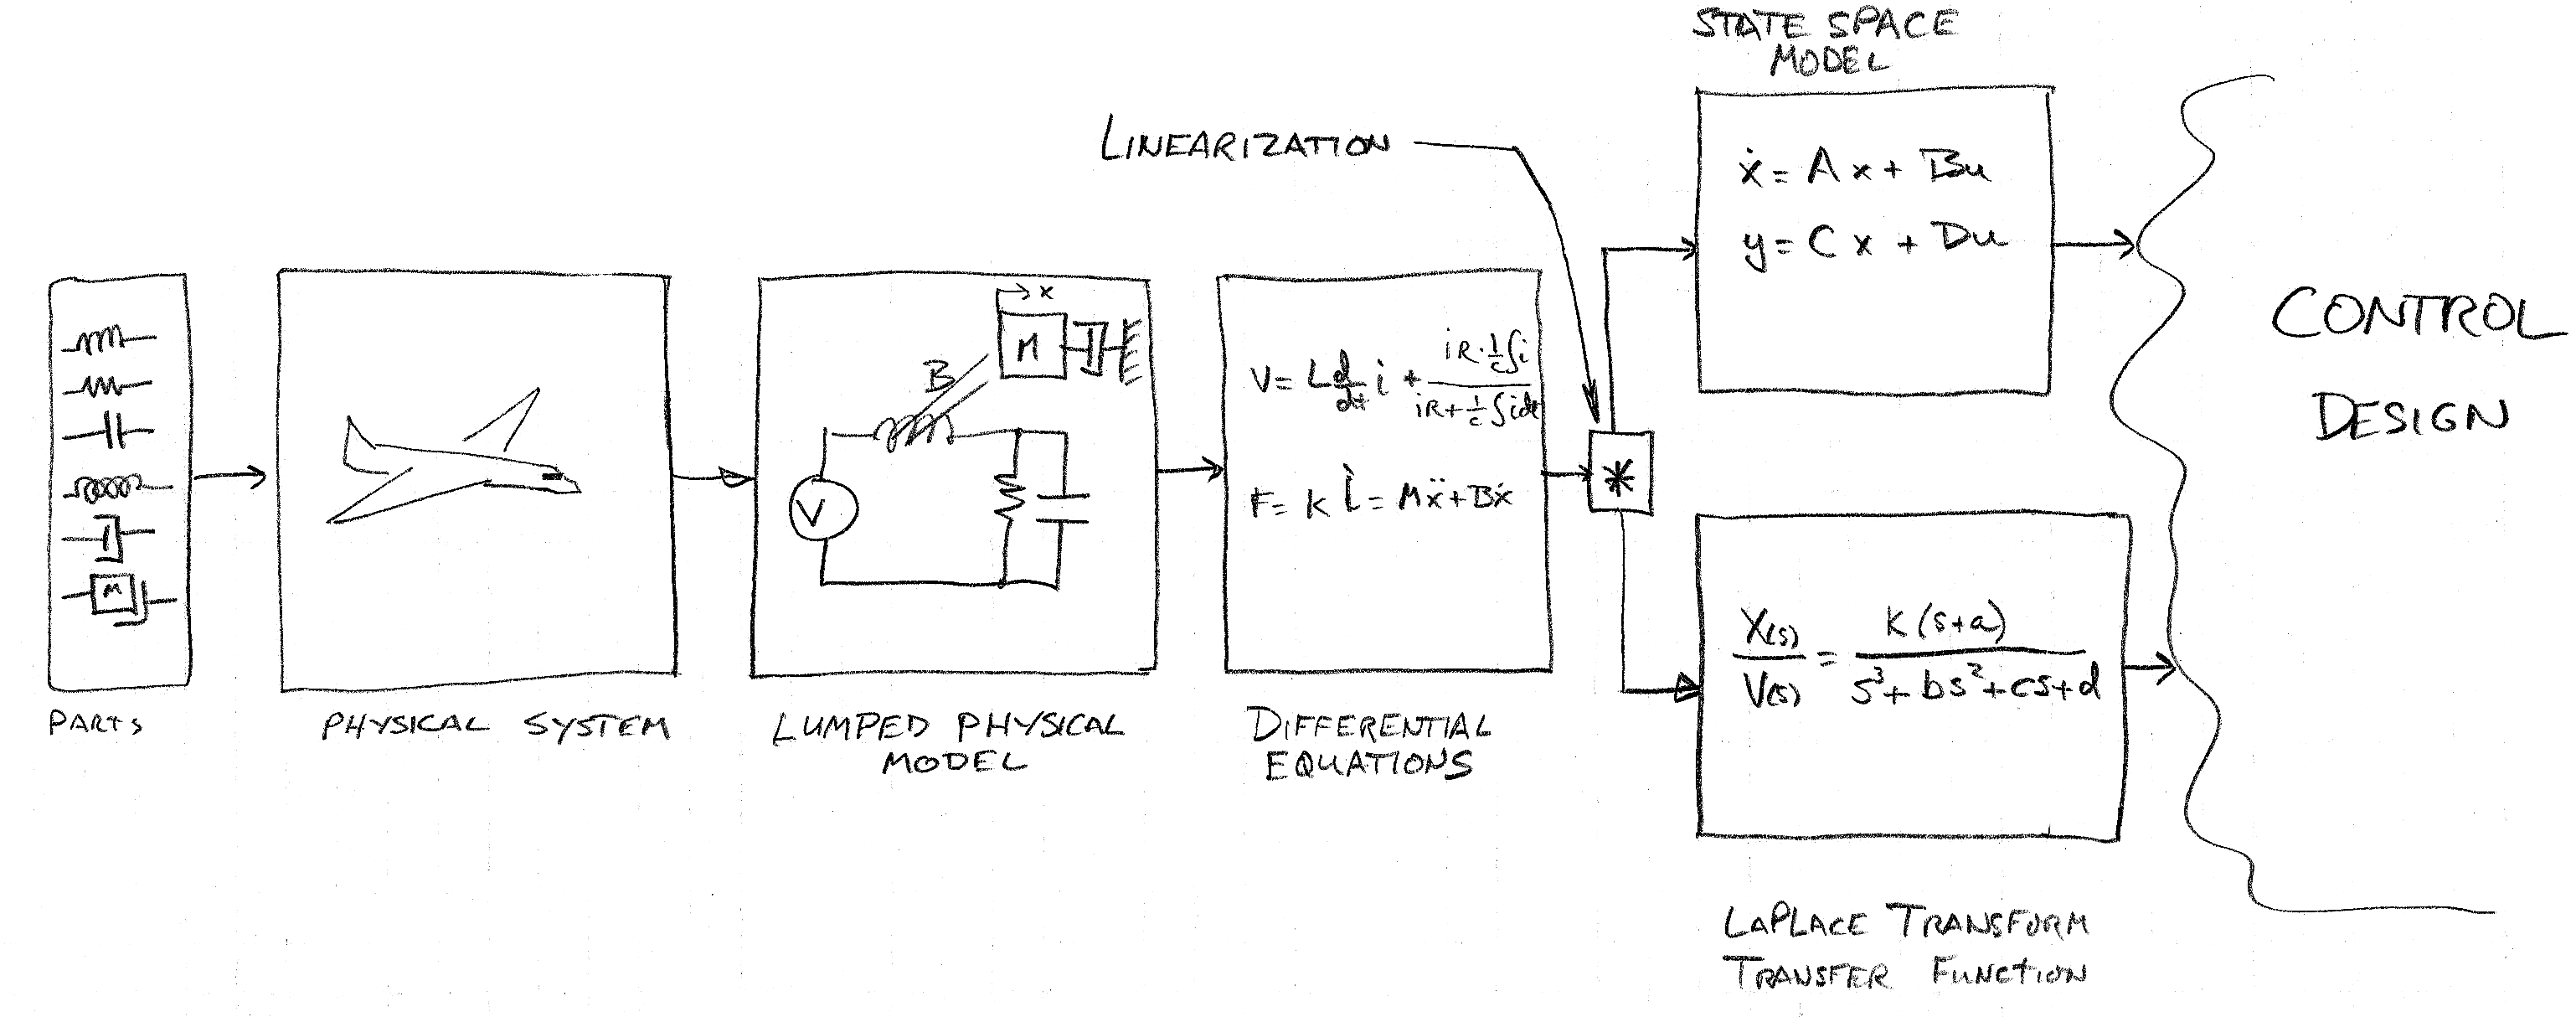
\includegraphics[width=6.45in]{figs01/01115.png}
\caption{Conceptual flow of system analysis preceding control system design.s}\label{fig_control_design_flow}
\end{figure}


%%%%** Section 2
\section{LODE}
%%%%** Section 2.1
\subsection{Basic definition}

A Linear Ordinary Differential Equation (LODE) is an equation of the form
\[
f(t) = \sum_{i=0}^{N} a_i\frac{d^i}{dt^i}x(t)
\]
The highest derivative, $N$, is referred to as the {\it order} of the LODE.  For example,
\[
f(t) = 0.273\frac{d^3}{dt^3}x(t) + 6.73\frac{d^2}{dt^2}x(t) - 0.001\frac{d}{dt}x(t) + 14.7x(t)
\]
is a third-order LODE.   Often we introduce some shorthand by omitting the time dependence ``$(t)$", and by using the dot notation for time derivatives:
\[
\dot{x} = \frac{d}{dt}x(t)  \qquad \ddot{x} = \frac{d^2}{dt^2}x(t)
\]
So that the example above would be written
\[
f(t) =0.273\frac{d^3}{dt^3}x + 6.73\ddot{x} - 0.001\dot{x} + 14.7x
\]
(you can use three dots for $\frac{d^3}{dt^3}$ if you wish.)



%%%%** Section 2.2
\subsection{Solution of First Order LODE}

A very basic  first order LODE is
\[
\dot{x} + Px = 0
\]

If we guess the solution is
\[
x(t) = e^{pt} \qquad \dot{x}(t) = pe^{pt}
\]
we can easily check it by plugging in to the original LODE:
\[
pe^{pt} +Pe^{pt} = 0 \to pe^{pt} = -Pe^{pt}
\]
giving
\[
p = -P
\]
so the solution is
\[
x(t) = e^{-Pt}
\]

Because of the partial fraction expansion (covered below), this covers a very wide variety of real world LODEs.


%%%%** Section 3
\section{Laplace Transform Review}

We will extensively use Laplace Transforms to manipulate the differential equations of control systems.  As a review, the Laplace transform is
\[
\sL \{f(t)\} = F(s) =  \int_{0}^{\infty} e^{-st}f(t)dt
\]
where $s$ is a complex variable, $s=\sigma + j \omega$.  Technically this is the ``one sided" Laplace Transform because the integral extends only to positive $t$.
The inverse of the Laplace Transform is
\[
f(t) = \sL^{-1}F(s) = \frac{1}{2\pi j} \lim_{T\to\infty} \int_{\sigma - j T}^{\sigma + jT}F(s) e^{st}ds
\]

For this course, we will not need to evaluate these integrals, because all of the LODEs we study will result in just a few terms which have been worked out long ago and are widely available in tables (Table \ref{LaplaceTransformTable}).



%%%%** Table 1
\begin{table}\centering
\renewcommand\arraystretch{2.0}% Vertical Row size, 1.0 is for standard spacing)
\begin{tabular}{|c|c|}
\hline
$ f(t)$ { for} $t \geq 0$ &  $\sL(f)$\\
\hline
$1u(t)$      & $\displaystyle \frac{1}{s}$\\\hline
$e^{at}$ & $\displaystyle \frac{1}{s-a}$\\ \hline
$t^n$    & $\displaystyle \frac{n!}{s^{n+1}}$ ($n = 0,1, \ldots$)\\ \hline
$\sin at$ & $\displaystyle \frac{a}{s^2 + a^2}$\\ \hline
$\cos at$ & $\displaystyle \frac{s}{s^2 + a^2}$\\ \hline
$\dot{f}(t)$ & $s{\cal L}(f)-f(0)$\\ \hline
$\ddot{f}(t)$ & $s^2{\cal L}(f)-sf(0)-\dot{f}(0)$
\\ \hline
\end{tabular}

(Where
$u(t) = \{ 0, t\le 0; 1, t > 0$,
$\dot{f}(t) = \frac{df(t)}{dt}$, $\ddot{f}(t) = \frac{d^2f(t)}{dt^2}$)
\caption{Table of some commonly used Laplace Transform pairs.}\label{LaplaceTransformTable}
\end{table}


When using this table we need to keep in mind a few limitations and assumptions:

\begin{itemize}
  \item We are only considering $t>0$.   One way to do this is to consider functions to be multiplied by the Unit Step function, $u(t)$

\[
  u(t) = \left \{ \begin{array}{ll}  0 & t < 0 \\ 1 & t > 0 \end{array} \right .
\]

  \item When using the differentiation relationship (last two lines of Table \ref{LaplaceTransformTable}) we must be careful about the initial conditions ($f(0), \dot{f}(0)$).    Most often, we assume that all initial conditions are zero, but it is your responsibility to verify that this assumption applies to a given problem.
\end{itemize}



%%%%** Example 1
\begin{ExampleSmall}
Find the Laplace Transform of the following time functions:  in all cases, assume the function is $0$ for $t<0$ and that initial conditions are zero

\vspace{0.2in}

\[
\sL\{55e^{-1.2t}\}
\]
Consulting the table and using the linearity property of the Laplace Transform integral:

\[
\sL\{55e^{-1.2t}\} = \frac {55} {s+1.2}
\]

\vspace{0.2in}
and

\[
\sL\{ 3.2\sin(7.6t) \} = \frac {24.32}{s^2 + 57.76}
\]
\vspace{0.2in}


\[
\sL\{ 2.6\ddot{x} - 3.52\dot{x} + 120x \} =
\]
\[
= 2.6X(s)s^2-3.52X(s)s+120X(s)
\]
\[
= X(s) \left(2.6s^2 - 3.52s + 120 \right)
\]
Note that we have assumed that $x(0) = \dot{x}(0) = \ddot{x}(0) = 0$.   Although this might seem restrictive, we often consider physical systems starting from rest (think rocket launch!) and this situation is well modeled by such zero initial conditions.
\end{ExampleSmall}


%%%%** Example 2
\begin{ExampleSmall}
Find the inverse Laplace transform of the following functions

\vspace{0.2in}

\[
\sL^{-1}\{\frac{10}{s+3.7}  \}
\]
Consulting the table and using the linearity property of the Laplace Transform integral:


\[
\sL^{-1}\{\frac{10}{s+3.7}  \}  = 10e^{-3.7t}
\]
\vspace{0.2in}
similarly

\[
\sL^{-1}\{ \frac{144s}{s^2 + 144} \}  = 144\cos(12t)
\]

\vspace{0.2in}


\[
\sL^{-1}\{ X(s)(s^3 + as^2 + bs+c) \} = \frac{d^3}{dt^3}x + a\ddot{x} + b\dot{x} + cx
\]

Here we have implicitly assumed zero initial conditions.

\end{ExampleSmall}


Let's apply the Laplace Transform to the initial LODE above.  First, we will modify the LODE to include a ``Forcing Function" on the right hand side.  A forcing function is typically a physical input to the system such as an applied voltage or force.

\[
\dot{x} + Px = f(t)
\]
Assuming zero initial conditions and taking the Laplace Transform of both sides (see the second to last line of Table \ref{LaplaceTransformTable}).
\[
sX(s) + PX(s) = F(s)
\]
\[
X(s) (s+P) = F(s)
\]
\[
\frac{X(s)}{F(s)} = \frac {1}  {(s+P)}
\]
Here we have derived a ratio called the ``Transfer Function" between position and the forcing function.  Our solution to the LODE was
\[
x(t) =  e^{pt} =  e^{-Pt}
\]
If we rewrite this using the solution, $p = -P$, then our transfer function becomes
\[
\frac{X(s)}{F(s)} = \frac {1}  {(s-p)}
\]
We call $p$ the ``pole" of this transfer function because the transfer function goes to infinity when $s=p$.



%%%%** Section 4
\section{Partial Fraction Expansion}\label{partialfractionsection}

A very useful property of polynomials is the partial fraction expansion:

\[
\frac{\prod_j (s-z_j)}{\prod_i (s-p_i)}    =  \sum_i  \frac{A_i}{(s-p_i)}
\]

In the form on the left, we have terms called $zeros$ on the top because any time $s=z_j$ the ratio is zero.  We also have terms called $poles$ in the denominator, because any time $s=p_i$, the ratio is infinite.

The partial fraction expansion is very useful for ratios of polynomials in $s$
(such as the left side above which we will encounter frequently) because such a ratio
becomes a series of terms which have an easy inverse Laplace Transform
\[
\frac{A_i}{(s-p_i)}   \leftrightarrow  A_ie^{p_it}
\]



\subsubsection{Single Poles Case}
For example,
\[
G(s) = \frac{s+5}{s^3 + 6s^2+ 358s+400}
\]
does not have an obvious inverse Laplace transform.   However if we can factor it to get

\[
G(s) = \frac  {(s+5)}   {(s+2)(s+4)(s+50)}
\]
then we can use the Partial Fraction expansion to  get it into the form
\[
G(s) = \frac{A_1}{(s+2)}+\frac{A_2}{(s+4)}+\frac{A_3}{(s+50)}
\]
then we can immediately write
\[
g(t) = A_1e^{-2t} + A_2e^{-4t} + A_3e^{-50t}
\]





It is not obvious that the partial fraction expansion is always possible but we will derive a class of cases and then perform some examples.
Let's call the exponential time constants
\[
p_1 = -2, \;p_2=-4,\; p_3 = -50
\]
and assume
\[
G(s) = \frac  {(s-z)}   {(s-p_1)(s-p_2)(s-p_3)} =  \frac{A_1}{(s-p_1)}+\frac{A_2}{(s-p_2)}+\frac{A_3}{(s-p_3)}
\]

Here we write $(s-p_1)$ because we usually are dealing with $negative$ real poles.   In other words: $(s+5) = (s - -5)$.   The real pole is $-5$ and the
term we are writing is $(s-p)$, where $p=-5$.

Now we multiply through by $(s-p_1)$:

\[
G(s) = \frac  {(s-p_1)(s-z)}   {(s-p_1)(s-p_2)(s-p_3)} =  \frac{A_1(s-p_1)}{(s-p_1)}+\frac{A_2(s-p_1)}{(s-p_2)}+\frac{A_3(s-p_1)}{(s-p_3)}
\]
Now we do two things:  1) cancel terms where possible,  2) solve for the special case $s=p_1$

\noindent
1)
\[
\frac  {(s-z)}   {(s-p_2)(s-p_3)} =  \frac{A_1}{1}+\frac{A_2(s-p_1)}{(s-p_2)}+\frac{A_3(s-p_1)}{(s-p_3)}
\]
2)
let $s=p_1$:
\[
\left . \frac  {(s-z)}   {(p_1-p_2)(p_1-p_3)} \right |_{s=p_1} =  \frac{A_1}{1}+\frac{A_2(p_1-p_1)}{(p_1-p_2)}+\frac{A_3(p_1-p_1)}{(p_1-p_3)}
\]
We can eliminate the $A_2,A_3$ terms! Giving:
\[
\frac  {(p_1-z)}   {(p_1-p_2)(p_1-p_3)} =  {A_1}
\]

Since everything on the left hand side is known,
we have just solved $A_1$.    If we multiply through by each denominator in turn, we can get all the $A_i$.




%%%%** Example 3
\begin{ExampleSmall}
Expand
\[
G(s) = \frac         {50(s+1)}                      {(s+0.1)(s+14)(s+567)}
\]
by the Partial Fraction Expansion.

\vspace{0.2in}
Solution:
\[
G(s) = \frac{A_1}{(s+0.1)} + \frac{A_2}{(s+14)} + \frac{A_3}{(s+567)}
\]

\[
A_1 = \left . \frac {(s+0.1)50(s+1)}{(s+0.1)(s+14)(s+567)} \right |_{s=-0.1} = \left . \frac {50(s+1)}  {(s+14)(s+567)}\right |_{s=-0.1}
\]
\[
= \frac {50(0.9)}{13.9\times566.9} = 0.00571
\]

\[
A_2 = \left . \frac {(s+14)50(s+1)}{(s+0.1)(s+14)(s+567)} \right |_{s=-14} = \frac {50(-13)}{-13.9 \times 553} = 0.0846
\]
\[
A_3 = \left . \frac {(s+567)50(s+1)}{(s+0.1)(s+14)(s+567)} \right |_{s=-567} = \frac {50(-566)}{-566.9 \times -553} = -0.090
\]
\vspace{0.15in}
\[
G(s) = \frac{0.00571}{(s+0.1)} + \frac{0.0846}{(s+14)} + \frac{-0.090}{(s+567)}
\]
\end{ExampleSmall}

%%%%** Example 4
\begin{ExampleSmall}
Use the Partial Fraction Expansion to find the inverse Laplace Transform of
\[
G(s) =  \frac          {27}             {(s+50)(s+3000)}
\]


\[
A_1 = \left . \frac {(s+3000)27}{(s+50)(s+3000)} \right |_{s=-3000} = \frac {27}{-2950} = -0.00915
\]
\[
A_2 = \left . \frac {(s+50)27}{(s+50)(s+3000)} \right |_{s=-50} = \frac {27}{2950} = 0.00915
\]

\[
g(t) = 0.00915(e^{-50t}-e^{-3000t})
\]

\end{ExampleSmall}



Sometimes the poles are complex conjugates\footnote{Recall that complex poles always come in complex conjugate pairs if our
system parameters such as $M,B,K,J,$ etc are real numbers.}, there are further simplifications possible after the Partial Fraction Expansion.




%%%%** Example 5
\begin{Example}

Find
\[
\sL^{-1}\{G(s) = \frac{(s+5)}{(s+6)(s+2+j)(s+2-j)}\}
\]

\vspace{0.25in}

Using the techniques above we can get:

\[
A_1 = -1/17 = -0.059 \qquad A_2 = 0.029+0.38j \qquad A_3 = 0.029-0.38j
\]
(note that it is not necessary to compute $A_3$ because it will always be the case for complex conjugate poles that $A_{n+1} = A_n^*$.)
\[
G(s)  = \frac {-0.059} {(s+6)}  + \frac {0.029+0.38j} {(s+2+j)}  + \frac {0.029-0.38j} {(s+2-j)}
\]

Applying the inverse transform to each term:

\[
g(t) = -0.059e^{-6t} + (0.029+0.38j)e^{(-2-j)t}+ (0.029-0.38j)e^{(-2+j)t}
\]

First, let's approximate
\[
0.029\pm 0.38j \approx 0.38e^{\pm j \pi/2}
\]
by 1) ignoring the small real part and
2) converting to Magnitude-Angle form (see Appendix \ref{ComplexNumberReview}).

\[
g(t) = -0.059e^{-6t} + 0.38e^{j\pi/2}e^{(-2-j)t} + 0.38e^{-j\pi/2}e^{(-2+j)t}
\]
\[
g(t) = -0.059e^{-6t} + 0.38e^{-2t} \left ( e^{j(-t+\pi/2)}+e^{-j(-t+\pi/2)} \right )
\]
Where we used:
\[
e^{j\pi/2}\cdot e^{(-2-j)t} \to e^{(j\pi/2-2t-jt)} \to e^{(-2t+j(\pi/2-t))} \to  e^{(-2t)}\cdot e^{j(\pi/2-t))}
\]
Now we use Euler's famous equality
\[
e^{j\theta} = \cos(\theta) + j \sin(\theta)
\]
as follows:
\[
g(t) = -0.059e^{-6t} + 0.38e^{-2t} \left (
    \cos(-t+\pi/2) + j\sin(-t+\pi/2)+
    \cos(-t+\pi/2) - j\sin(-t+\pi/2)
    \right )
\]
Since $\cos(\theta) = -\cos(\theta)$, and $\cos(\theta-/pi/2) = \sin(\theta)$

\[
g(t) = -0.059e^{-6t} + 0.38e^{-2t} \left (
    2\cos(t-\pi/2)
    \right )
\]
\[
g(t) = -0.059e^{-6t} + 0.76e^{-2t} \left (
    \cos(t-\pi/2)
    \right )
\]
\[
g(t) = -0.059e^{-6t} + 0.76e^{-2t} \left (  \sin(t)  \right )
\]

\end{Example}



%%%%** Example 5
\begin{ExampleCont}
By throwing a few values of $t$ into the calculator, we can generate a sketch of the second term as shown below:
$ 0.76e^{-2t} \left (  \sin(t)  \right )$

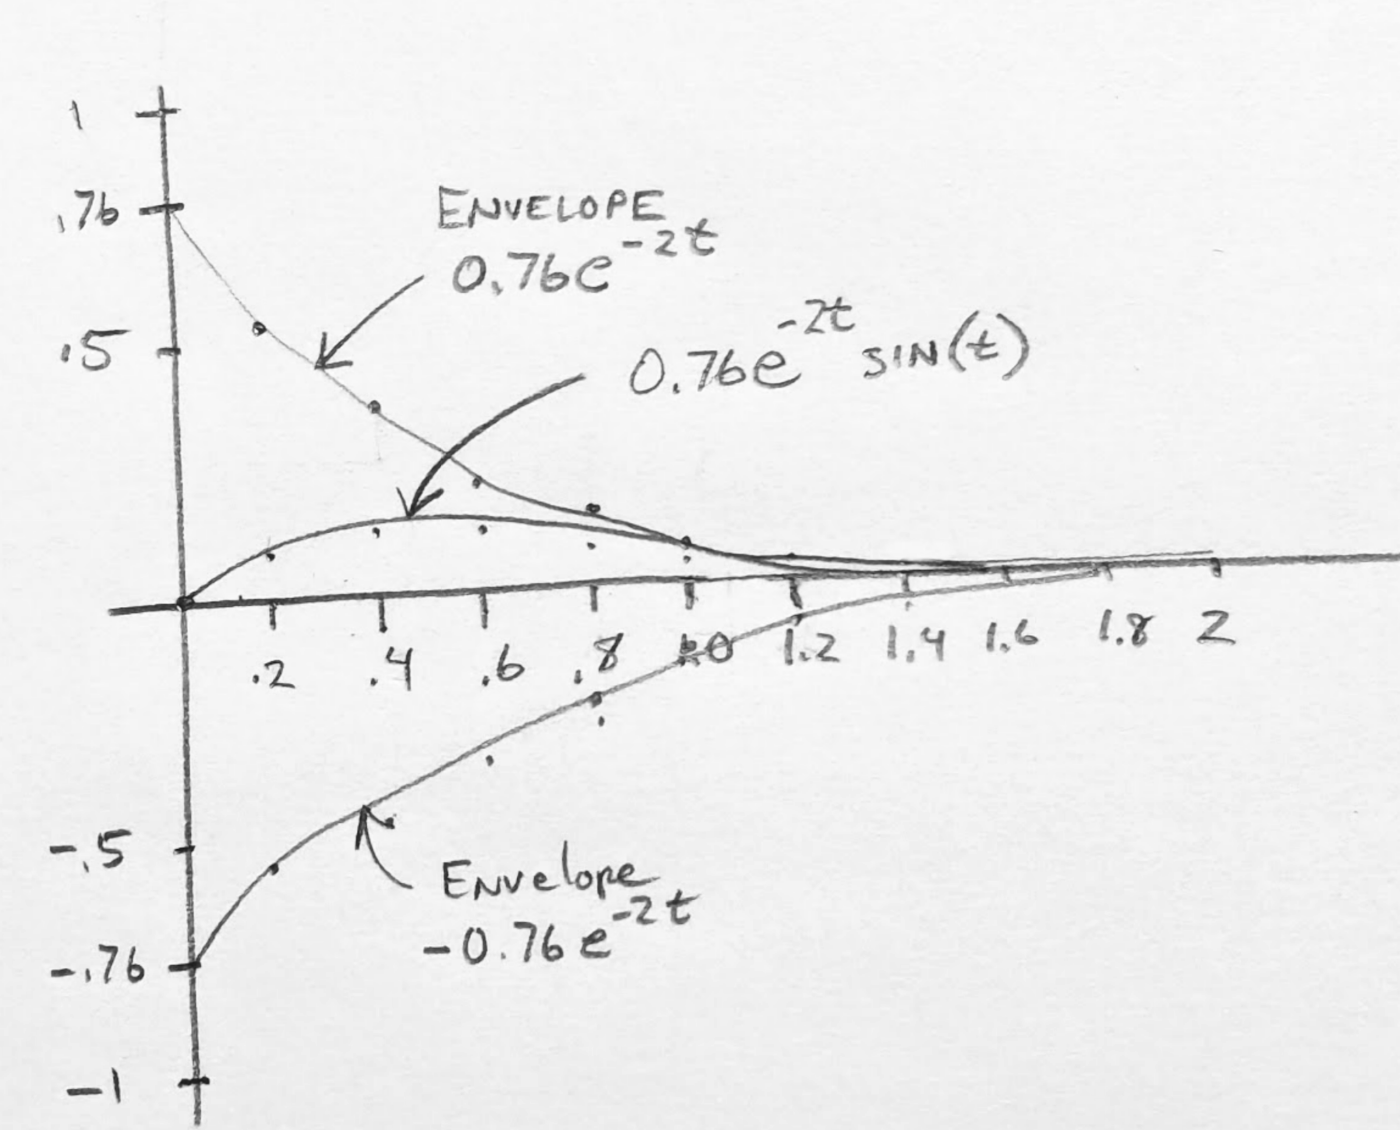
\includegraphics[width=82mm]{figs01/J55Q14.png}

For a more accurate plot, let's use the computer on the final result(including both terms):
\[
g(t) = -0.059e^{-6t} + 0.76e^{-2t} \left (  \sin(t)  \right )
\]

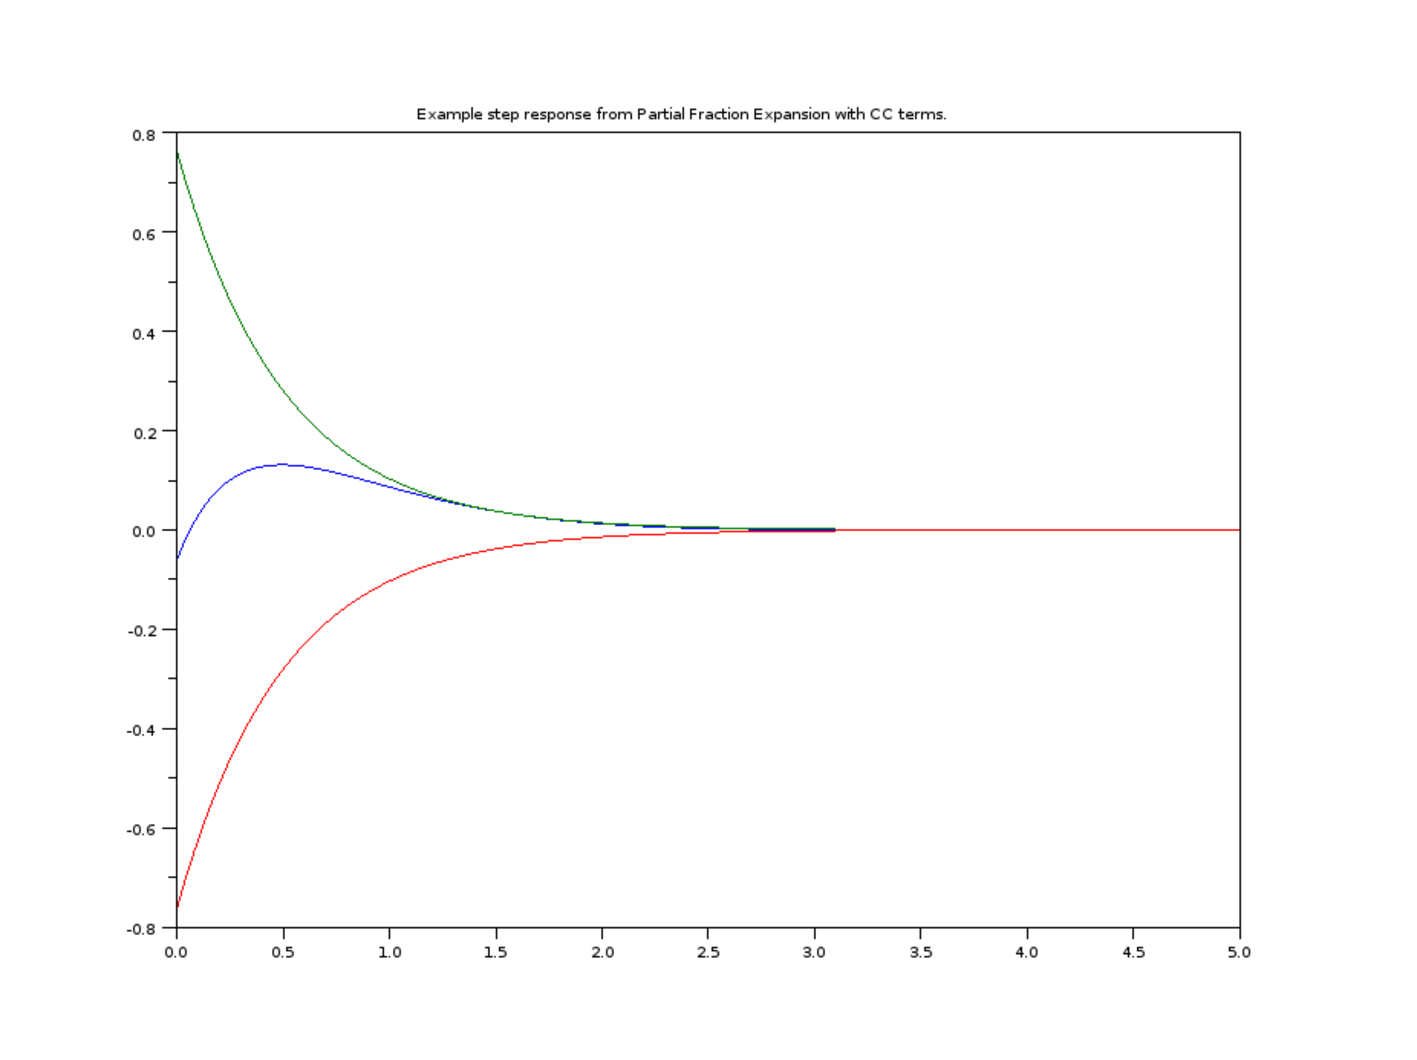
\includegraphics[width=120mm]{figs01/pf_compConja.png}


\end{ExampleCont}

\subsubsection{Repeated Poles}

Another situation comes when a pole is repeated (i.e. $\frac{1}{(s+2)^2}$).  In this case the trick we use for the partial fraction expansion no longer works!   But instead we can still solve for $A_i$ by differentiating the partial fraction expansion.

%%%%** Example 6
\begin{ExampleSmall}
Apply the Partial Fraction Expansion to
\[
G(s) = \frac {(s+5)}  {s^2(s+3)}
\]
(note that there is a repeated root  in the demoninator (repeated pole at $s=0$)).

We start by setting up the problem with two terms for the repeated pole:

\[
G(s) = \frac {A_1}{s^2} +  \frac {A_2}{s} +  \frac {A_3}{(s+3)}
\]
$A_1$:

\begin{equation}\label{eqn1Ex1p6}
\left . \frac{s^2(s+5)} {s^2(s+3)}\right |_{s=0}  = \frac {s^2A_1}  {s^2}   + \frac{s^2A_2} {s} + \frac {s^2A_3} {(s+3)}
\end{equation}
giving
\[
A_1 = 5/3
\]

$A_3$ is also straightforward, giving $A_3 = 2/9$. But working through $A_2$ we find:

\[
\left . \frac{s(s+5)} {s^2(s+3)}\right |_{s=0}  = \frac {sA_1}  {s^2}   + {A_2}  + \frac {sA_3} {(s+3)}
\]

We now have the problem that we cannot cancel the $s^2$ in the denominator of the $A_2$ term (which we need to do!).   Instead differentiate the $A_1$ expression (Eqn. \ref{eqn1Ex1p6} with respect to $s$:
\[
\frac{d}{ds}\frac{(s+5)}{(s+3)} = 0 + A_2 + \frac{d}{ds} \frac{s^2}{(s+3)}A_3
\]
Using an advanced differentiation rule (below) gives:
\[
\frac{-2}{(s+3)^2} = A_2 + \frac{s(s+6)}{(s+3)^2}A_3
\]
evaluating at $s=0$,
\[
A_2 = -2/9
\]
The tricks we used used:
\[
\frac{d}{dx}\frac{(x+a)}{(x+b)} = \frac{1}{(x+b)} - \frac{(x+a)}{(x+b)^2}
\]
and
\[
\frac{d}{dx} \frac{x^2}{(x+a)} = \frac{2x}{(x+a)} - \frac{x^2}{(x+a)^2}
\]

This gets even more unwieldy when the repeated pole is non-zero, but fortunately we rarely need this technique or can fall back on numerical
or AI-based symbolic methods.
\end{ExampleSmall}




%%%%** Section 5
\section{Linearization}

\subsection{Overview}
Laplace Transforms can only be used on linear equations.  In most of this course we focus on linear differential equations but often real world applications involve non-linear functions.   All is not lost if we can usefully {\it approximate} our non-linear function with a linear one.  Our approach to linearization is to model the original function with a straight line.


Consider a nonlinear function, $f(x)$.  The linearized version of $f(x)$, $\hat{f}(x)$,  can be constructed about a specific operating point, $x_0$.

\[
\hat{f}(x) = f(x_0) + \frac{d}{dx}f(x_0) (x-x_0)
\]

$\hat{f}(x)$ is a linear function of $x$ which is most accurate in the neighborhood of $x_0$.   It is also the  first two terms of a Taylor series expansion of $f(x)$.   It is very helpful to visualize this process graphically by plotting the linearized function on top of the original function (Figure \ref{locallinearizationSketch}).

\begin{figure}\label{locallinearizationSketch}
  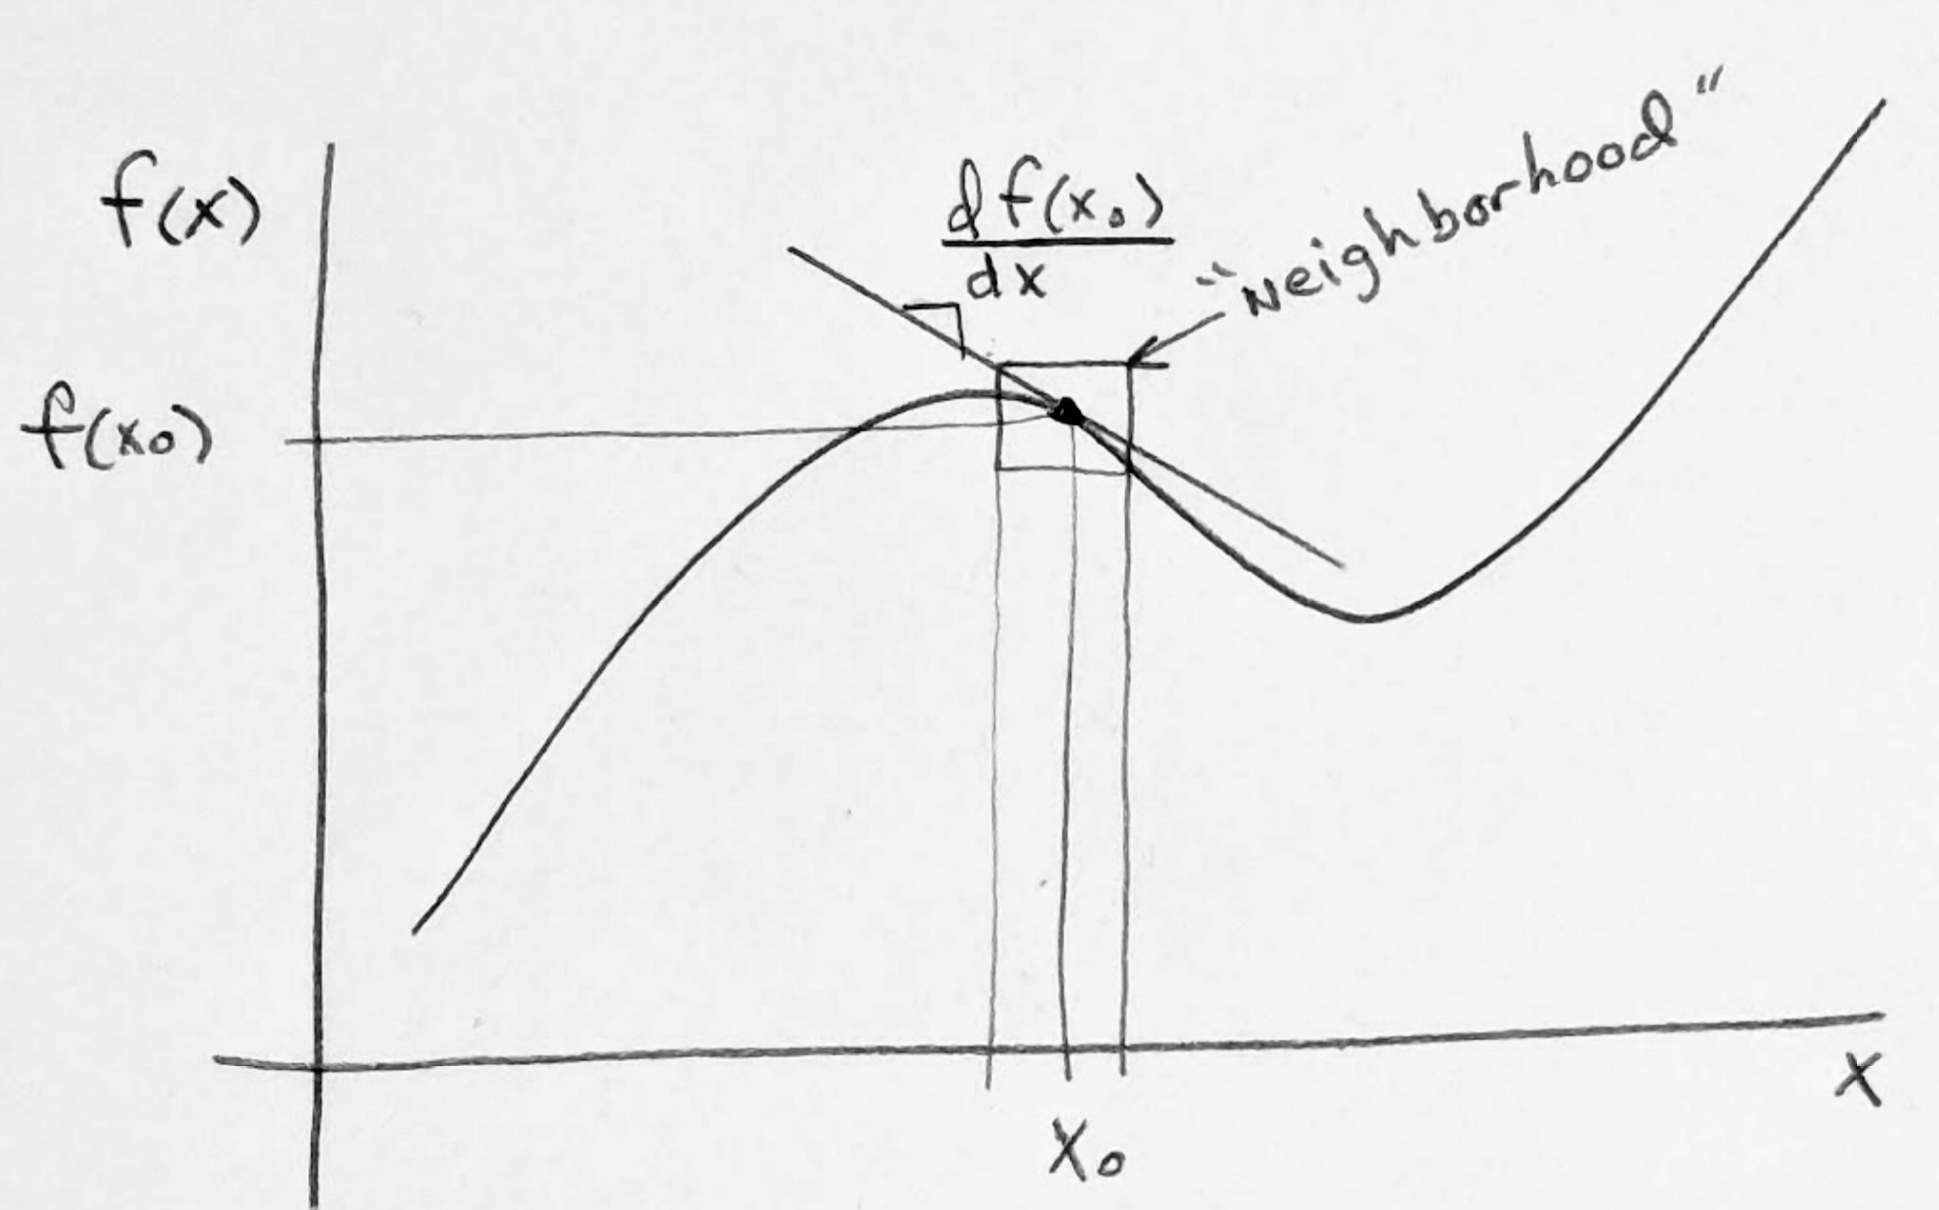
\includegraphics[width=105mm]{figs01/Q75B05.png}
  \caption{Illustration of a linearized version of a non-linear function at an operating point.}
\end{figure}
\clearpage



\subsection{Linearization Examples}
%%%%** Example 7
\begin{ExampleSmall}\label{twolinexamples}

Consider the nonlinear function
\[
f_1(x) = 0.4x^2 -0.1x^3 + 3\sin(x)
\]
and linearize twice, once about $x=-6$, and again about $x=1$ (we are using radians for $\sin(x)$).

\vspace{0.2in}

First evaluate $f_1(x)$ for the two linearization points:
\[
f_1(-6) = 36.84 \qquad  f_1(1) = 2.824
\]
Then let's get the derivative:

\[
\dot{f}(x) = 0.8x -0.3x^2 +3\cos(x)
\]
and evaluate it at the two points:

\[
\dot{f}(-6) = -12.72 \qquad \dot{f}(1) = 2.121
\]

Now we get:

\[
\hat{f}_{1a} = 36.84-12.72(x+6) = -39.48-12.72x \qquad \hat{f}_{1b} = 2.824+2.121(x-1) = 0.703+2.121x
\]

Plotting using the computer:
\begin{center}
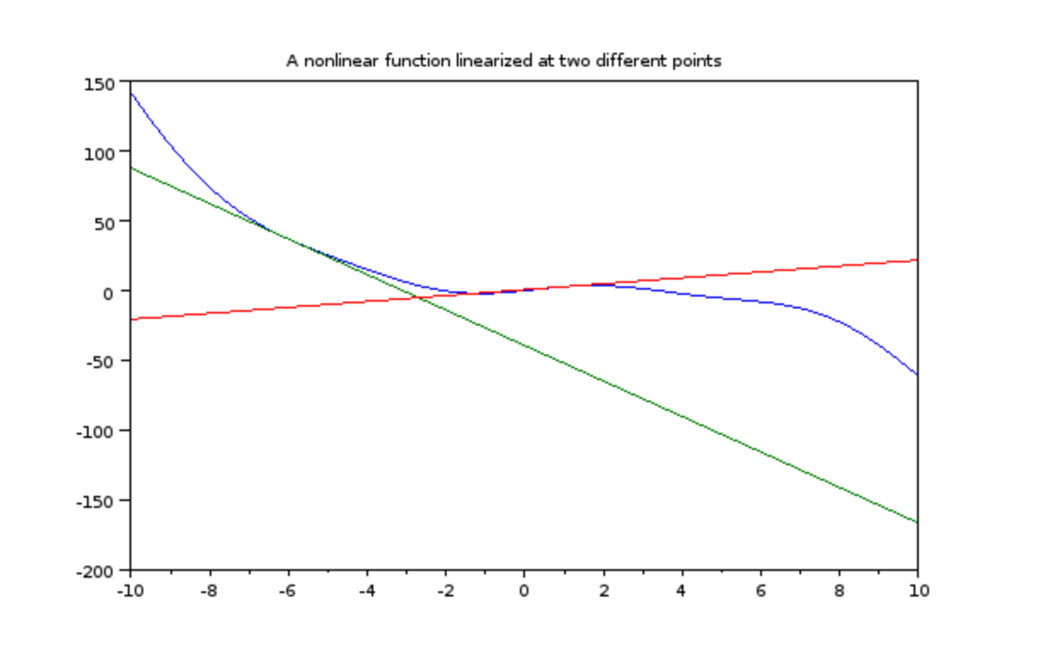
\includegraphics[width=3.5in]{figs01/linearizeattwopointsa.png}
\end{center}

The blue line is $f(x)$, the green line is $\hat{f}_{1a}(x)$ and the red line is $\hat{f}_{1b}(x)$.  The linear approxmations are reasonably accurate in the neighborhood of their operating points ($x = -6, +1$), but become very bad as we move away.  The size of the ``neighborhood" for which a degree of accuracy can be obtained depends on the function and the selected operating point.

\end{ExampleSmall}


Some combinations of functions and operating points are especially easy to linearize.

%%%%** Example 8
\begin{ExampleSmall}
Linearize
\[
f_2(x) = 0.723x^3 -4.37x^2 +67x
\]
about the point $x=0$
\vspace{0.2in}

\[
f_2(0) = 0
\]
\[
\frac{d}{dx}{f}_2(x) = 2.169x^2 - 8.74x + 67
\]
\[
\frac{d}{dx}{f}_2(0) = 67
\]
\[
\hat{f}_2(x) =  67x
\]
Note that we are simply taking the linear term of $f_2(x)$, $67x$.
However we only could get away with this because 1) we linearized about $x=0$ and 2) the function was a polynomial.
\end{ExampleSmall}

%%%%** Example 9
\begin{ExampleSmall}
Linearize $f_2(x)$ from the previous example about $x=5.7$
\vspace{0.2in}

\[
f_2(5.7) = 373.81
\]
\[
\frac{d}{dx}{f}_2(5.7) = 87.6521
\]
\[
\hat{f}_{2a}(x) = 373.81 + 87.6521(x-5.7)
\]
\[
\hat{f}_{2a}(x) = -125.81 + 87.6521x
\]
This is quite different from $\hat{f}_2(x)$.  So only if we carefully use the two rules of the previous example, we
can linearize by simply deleting all terms except the linear term.

\end{ExampleSmall}


When the equation to be linearized is a differential equation,
% we introduce a slightly strange notion: taking the derivative with respect to a derivative:
just

\begin{enumerate}
  \item isolate the non-linear part
  \item treat it like a simple function
  \item linearize the function
  \item plug the function back into the differential equation
\end{enumerate}

%%%%** Example 10
\newpage\begin{ExampleSmall}
Linearize the differential equation
\[
f_3(t) =   \ddot{x} - 0.42\dot{x} + 0.01(\dot{x})^3 + \sin(5\dot{x}) + 16x
\]
about $\dot{x} = 0$  (We have omitted $(t)$ from $\{x(t), \dot{x}(t),\ddot{x}(t)\}$ to simplify notation.)
$\dot{x}$ is often the velocity of a physical part.
Does a system do anything interesting if $\dot{x} = 0$?  It can.  Remember the linearization works
in the {\it neighborhood} of the operating point -- so we could say this linearization is valid for slow speeds
(velocities near zero).  That might be what we care about in our application.


\vspace{0.2in}
The nonlinear part of this differential equation can be taken out as a simple function, $Fn()$:
\[
Fn(y) = 0.01y^3+\sin(5y)
\]
where we are using the variable $y$ just to avoid confusion with $x,\dot{x}$.   Now we linearize $Fn(y)$ about $y=0$:
\[
\frac{d} {dy}Fn(y)  = 0.03y^2+5\cos(5y)
\]
\[
\hat{F}n(y) = Fn(0) + \left . \frac{d} {dy}Fn(y) \right|_{y=0} (y-0) = 0 + 5\cos(0)y = 5y
\]\[
\hat{F}n(y) = 5y
\]
Plugging the linearized function back into the differential equation:
\[
f_3(t) =   \ddot{x} - 0.42\dot{x} + \hat{F}n(\dot{x}) + 16x
\]
\[
f_3(t) =   \ddot{x} - 0.42\dot{x} + 5\dot{x} + 16x = \ddot{x} + 4.58\dot{x} + 16x
\]
This LODE is a linearized version of our system which is valid in the neighborhood of $\dot{x}=0$ (i.e. for low velocities).
\end{ExampleSmall}


\subsection{Range of Approximation}
We have seen that linearization ``works" ``in the neighborhood" of the linearization point.   Here we will dive deeper into what
we mean by ``works" and ``neighborhood".

First we must define our requirement for accuracy (i.e. how much error we can have while the approximation still ``works").
Often this is dictated by some external requirement.  For example,
\begin{quotation}
The linearized model shall have less than 10\% error.
\end{quotation}
By this we mean that if we define a linear function $\hat{f}(x)$ which is a linear approximation of a non-linear function,
$f(x)$, about the point $x = x_0$ then
\[
\frac   {|f(x)-\hat{f}(x)| } {f(x)} < 0.10
\]
% We choose $f(x_0)$ as the denominator since it defines the scale for our local function.

Second, we must define ``neighborhood".    By this we mean the range of $x$ values for which the approximation is good enough (i.e. ``works").   Suppose we have
\[
x_{min} < x_0 < x_{max}
\]
such that

\[
\frac   {|f(x_{min})-\hat{f}(x_{min})| } {f(x_{min})} = 0.10
\]
and

\[
\frac   {|f(x_{max})-\hat{f}(x_{max})| } {f(x_{max})} = 0.10
\]

Assuming that $f(x)$ changes slowly, we can call the ``neighborhood"
\[
x_{min} < x < x_{max}
\]
the region where the approximation is sufficient.



\begin{Example}
Consider the system of Example \thechapter.\ref{twolinexamples}.  The equations were:

\[
f_1(x) = 0.4x^2 -0.1x^3 + 3\sin(x)
\]
 linearized twice, once about $x=-6$ radians, and again about $x=1$ radian.


\[
\hat{f}_{1a} =  -39.48-12.72x \qquad \hat{f}_{1b} =  0.703+2.121x
\]

If the accuracy requirement is 5\%, which linearization $a$ or $b$ has a bigger ``neighborhood"?


Our approach will be to compute numerically values of $f(x)$ and $\hat{f}(x)$ and look for the error dropping below 5\%
We'll define our error percentage as:
\[
E_j = \left| \frac {f(x) - f_j(x)} {f(x)}  \right |
\]

Let's make a spreadsheet for them both.  We'll generate columns as follows:

\begin{tabular}{|c|c|c|c|c|c|}\hline
A & B & C & D & E & F \\ \hline
$x$  & $f_1(x)$ & $f_{1a}(x) $  &  $E_a$ & $f_{1b}(x) $ &  $E_b$ \\
\hline
\end{tabular}


\begin{tabular}{cp{0.4\textwidth}}
\begin{minipage}{0.45\textwidth}
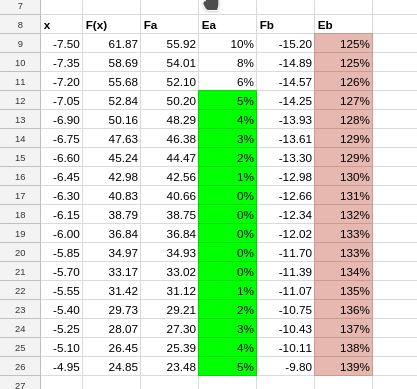
\includegraphics[width=\textwidth]{figs01/lin_sheet_01.png}
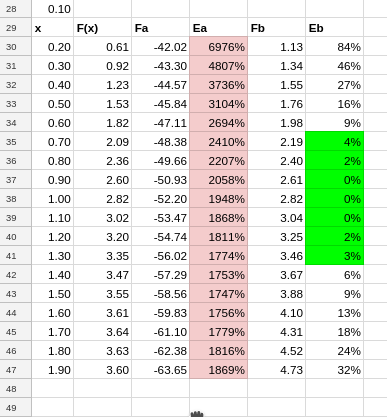
\includegraphics[width=\textwidth]{figs01/lin_sheet_02.png}
\end{minipage}

&

\begin{minipage}{0.45\textwidth}
\begin{center}
{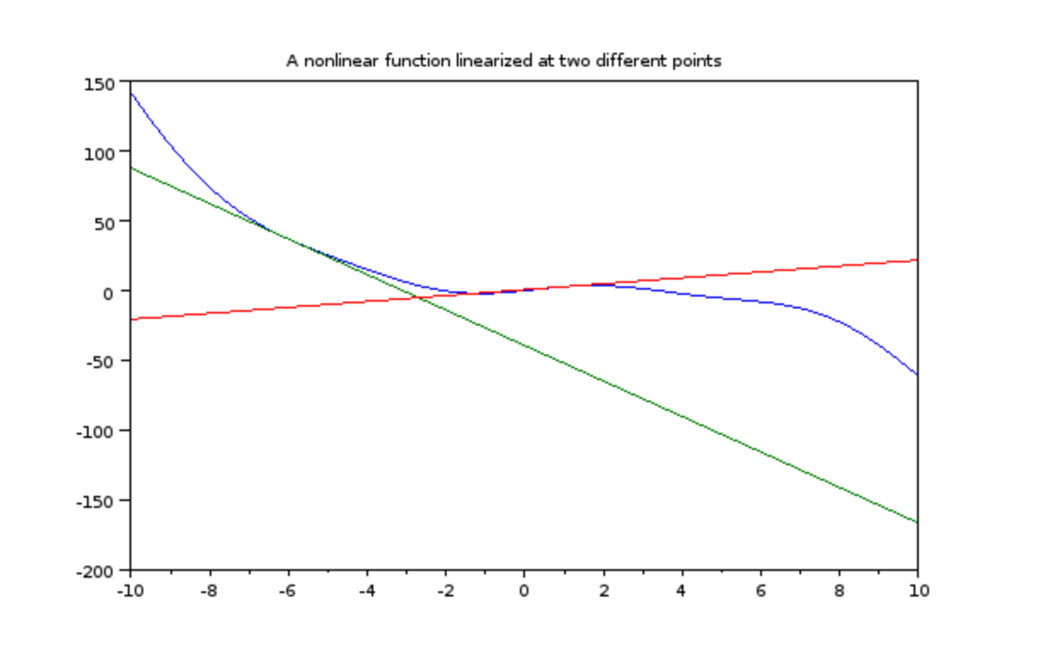
\includegraphics[width=\textwidth]{figs01/linearizeattwopointsa.png}}
\end{center}

There are two sets of rows, one centered around each linearization point ($x=-6$, and $x=1$).
Colors indicate good and bad accuracy.  The green box shows the $\pm5\%$ zone.  Note how
$f_{1a}$ is accurate near $x=-6$ and $f_{1b}$ is accurate near $x=1$.

Answering our specific question, the range for $f_{1a}$ is
\[
-7.04 < x < -4.95 =  2.09
\]
and for $f_{1b}$
\[
0.70 < x < 1.30 = 0.6
\]
So $f_{1a}$ has a bigger ``neighborhood".    However we are usually forced to pick the linearization point from
an application requirement so in the real world we can't just choose our linearization point according to how well linearization fits. For example, if a model of room climate control requires linearization, we MUST linearize about $T=70^\circ F$ or something close to that because we have to operate in the range of human comfort.
\end{minipage}

\vspace{0.35in}



\end{tabular}

\end{Example}





























% \section{Summary of Notation}

